\newpage
\sect{OBS /OBS Studio Einrichten}

% \sub{Stream planen}

{\vspace{0.2cm}}
\begin{center}
  \textbf{Hierfür klickt hierfür auf \quote{Stream planen } rechts oben.} \\
  {\vspace{0.3cm}}
  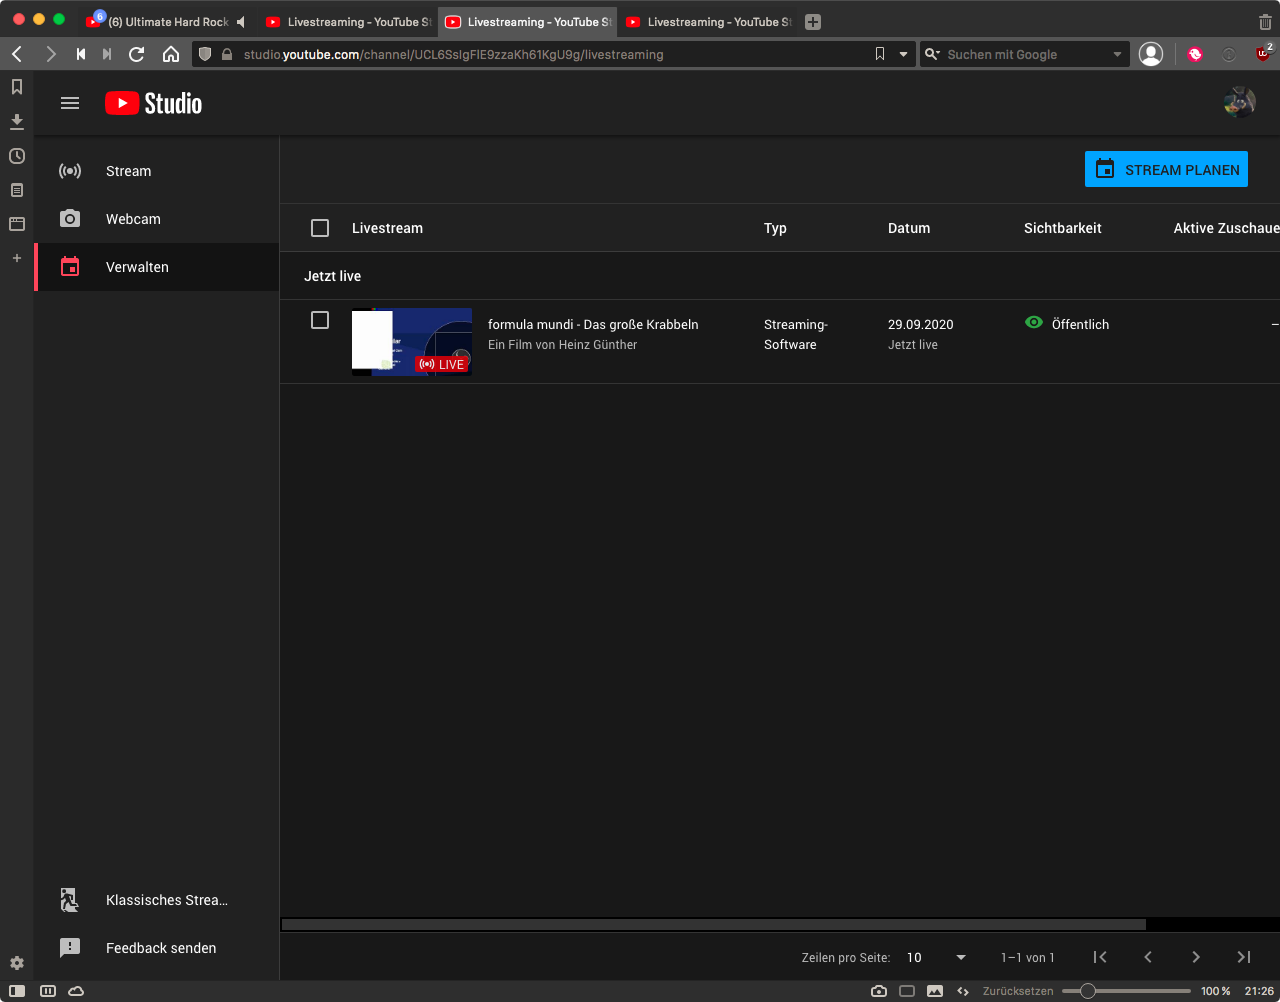
\includegraphics[width=0.7\textwidth]{./pictures/YOUTUBEstreamPlanen1.png}
\end{center}



% {\vspace{-0.6cm}}
\begin{center}
  \textbf{Hier ist es wichtig die Zielgruppeneinstellung zu setzen.} \\
  {\vspace{0.3cm}}
  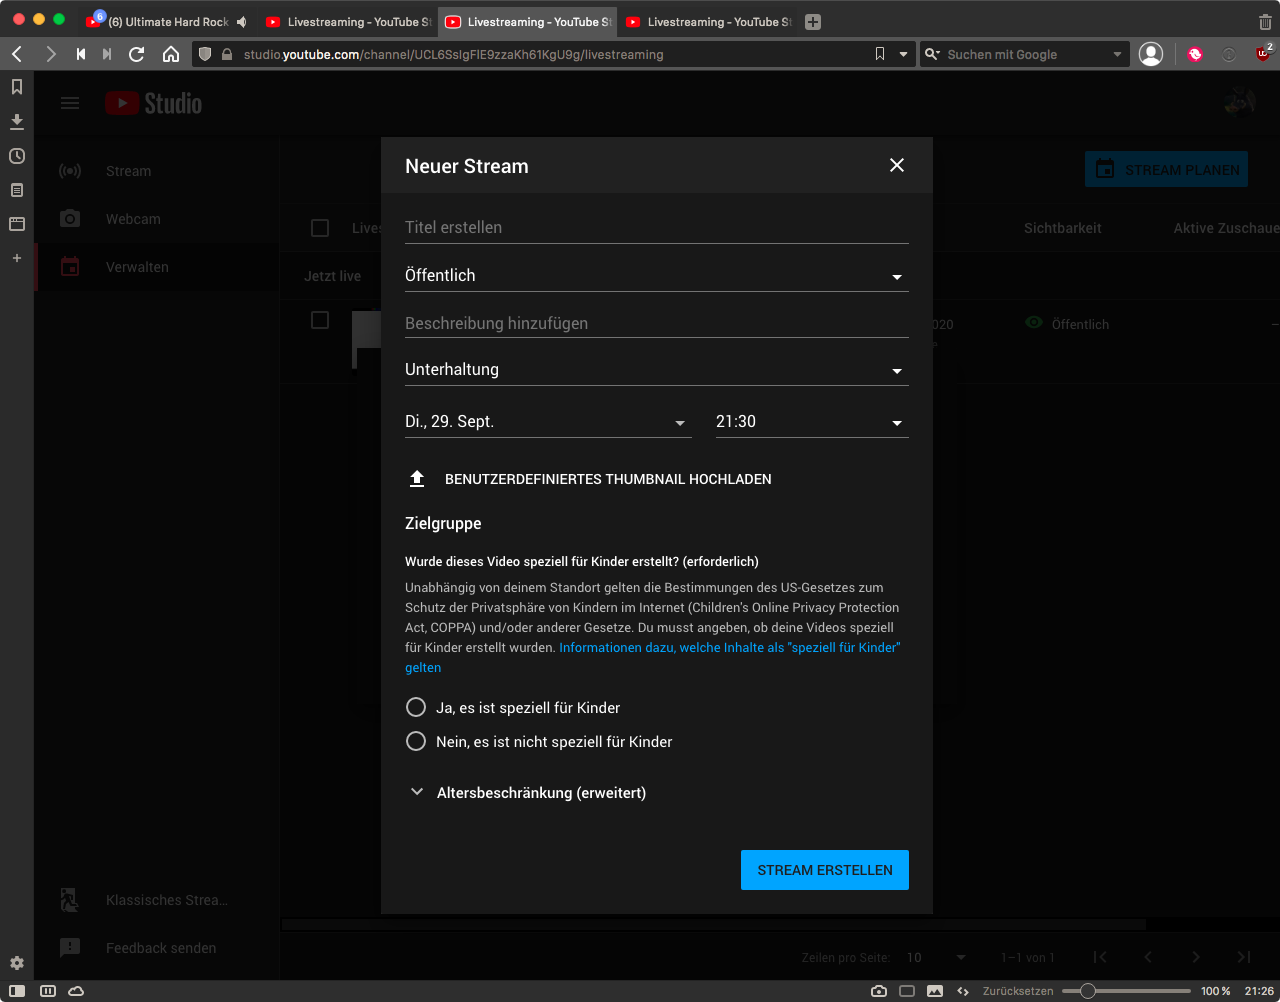
\includegraphics[width=0.7\textwidth]{./pictures/YOUTUBEstreamPlanen2.png}
\end{center}

\newpage
% {\vspace{-0.6cm}}
\begin{center}
  \textbf{In den Stream Einstellungen kann man nun die Latenz Einstellen und bekommt den Stream-Schlüssel für OBS} \\
  {\vspace{0.3cm}}
  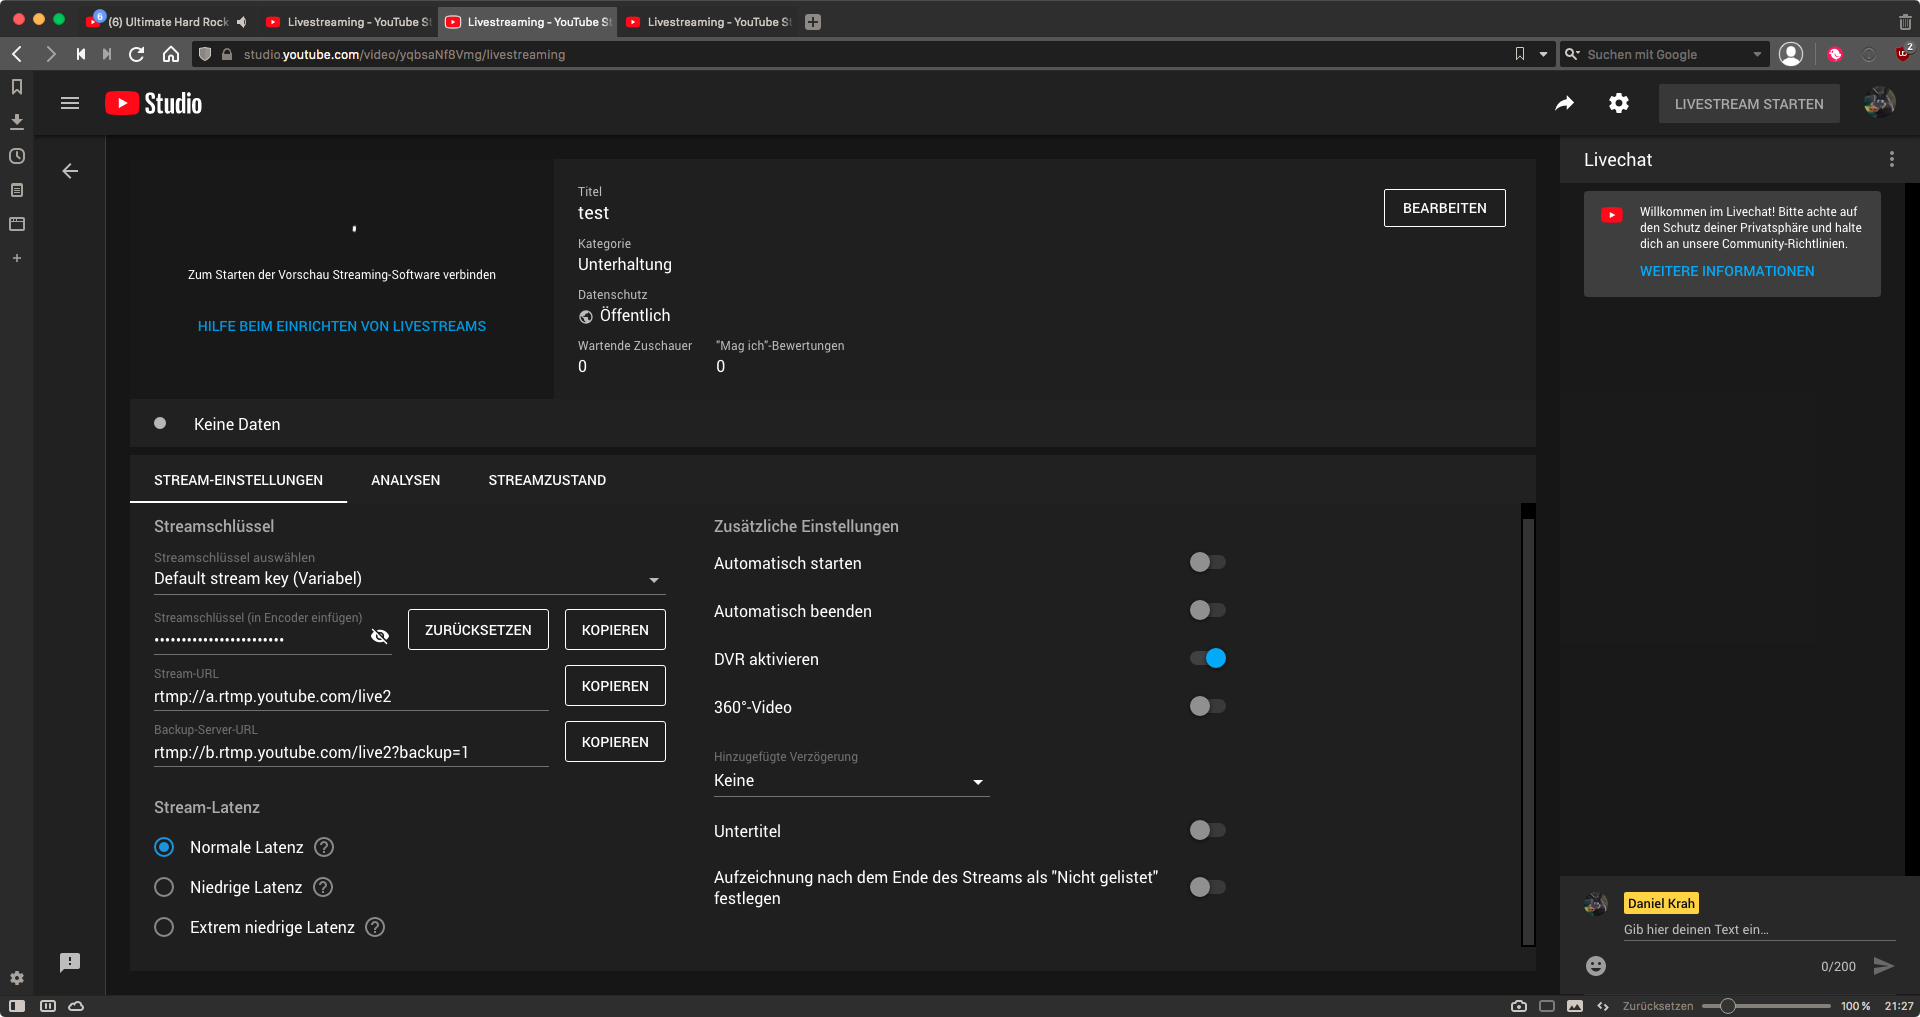
\includegraphics[width=0.9\textwidth]{./pictures/YOUTUBEstreamPlanen3.png}
\end{center}

% {\vspace{-0.6cm}}
\begin{center}
  \textbf{Diesen kann man nun in OBS unter Stream eintragen} \\
  {\vspace{0.3cm}}
  \includegraphics[width=0.7\textwidth]{./pictures/schlüsselEingetragen.png}
\end{center}

\newpage
% {\vspace{-0.6cm}}
\begin{center}
  \textbf{Es müssen als Nächstes die Datenraten für Audio und Video gesetzt werden ...} \\
  {\vspace{0.3cm}}
  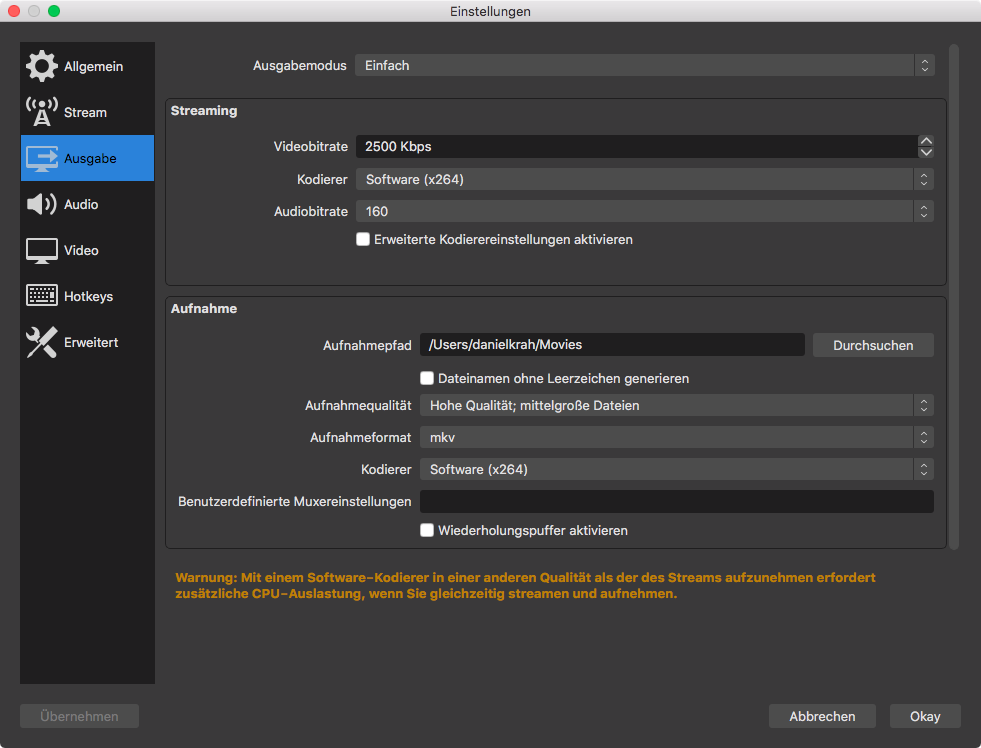
\includegraphics[width=0.7\textwidth]{./pictures/configDatenRate.png}
\end{center}

% {\vspace{-0.6cm}}
\begin{center}
  \textbf{... Sowie die Auflösung für den Videostream} \\
  {\vspace{0.3cm}}
  \includegraphics[width=0.7\textwidth]{./pictures/configAuflösung.png}
\end{center}



\newpage
% {\vspace{-0.6cm}}
\begin{center}
  \textbf{In beiden Programmen können Filme als Videoquelle sowie Webcams eingebunden werden} \\
  \textbf{Ebenso sind Hintergründe möglich.} \\
  {\vspace{0.3cm}}
  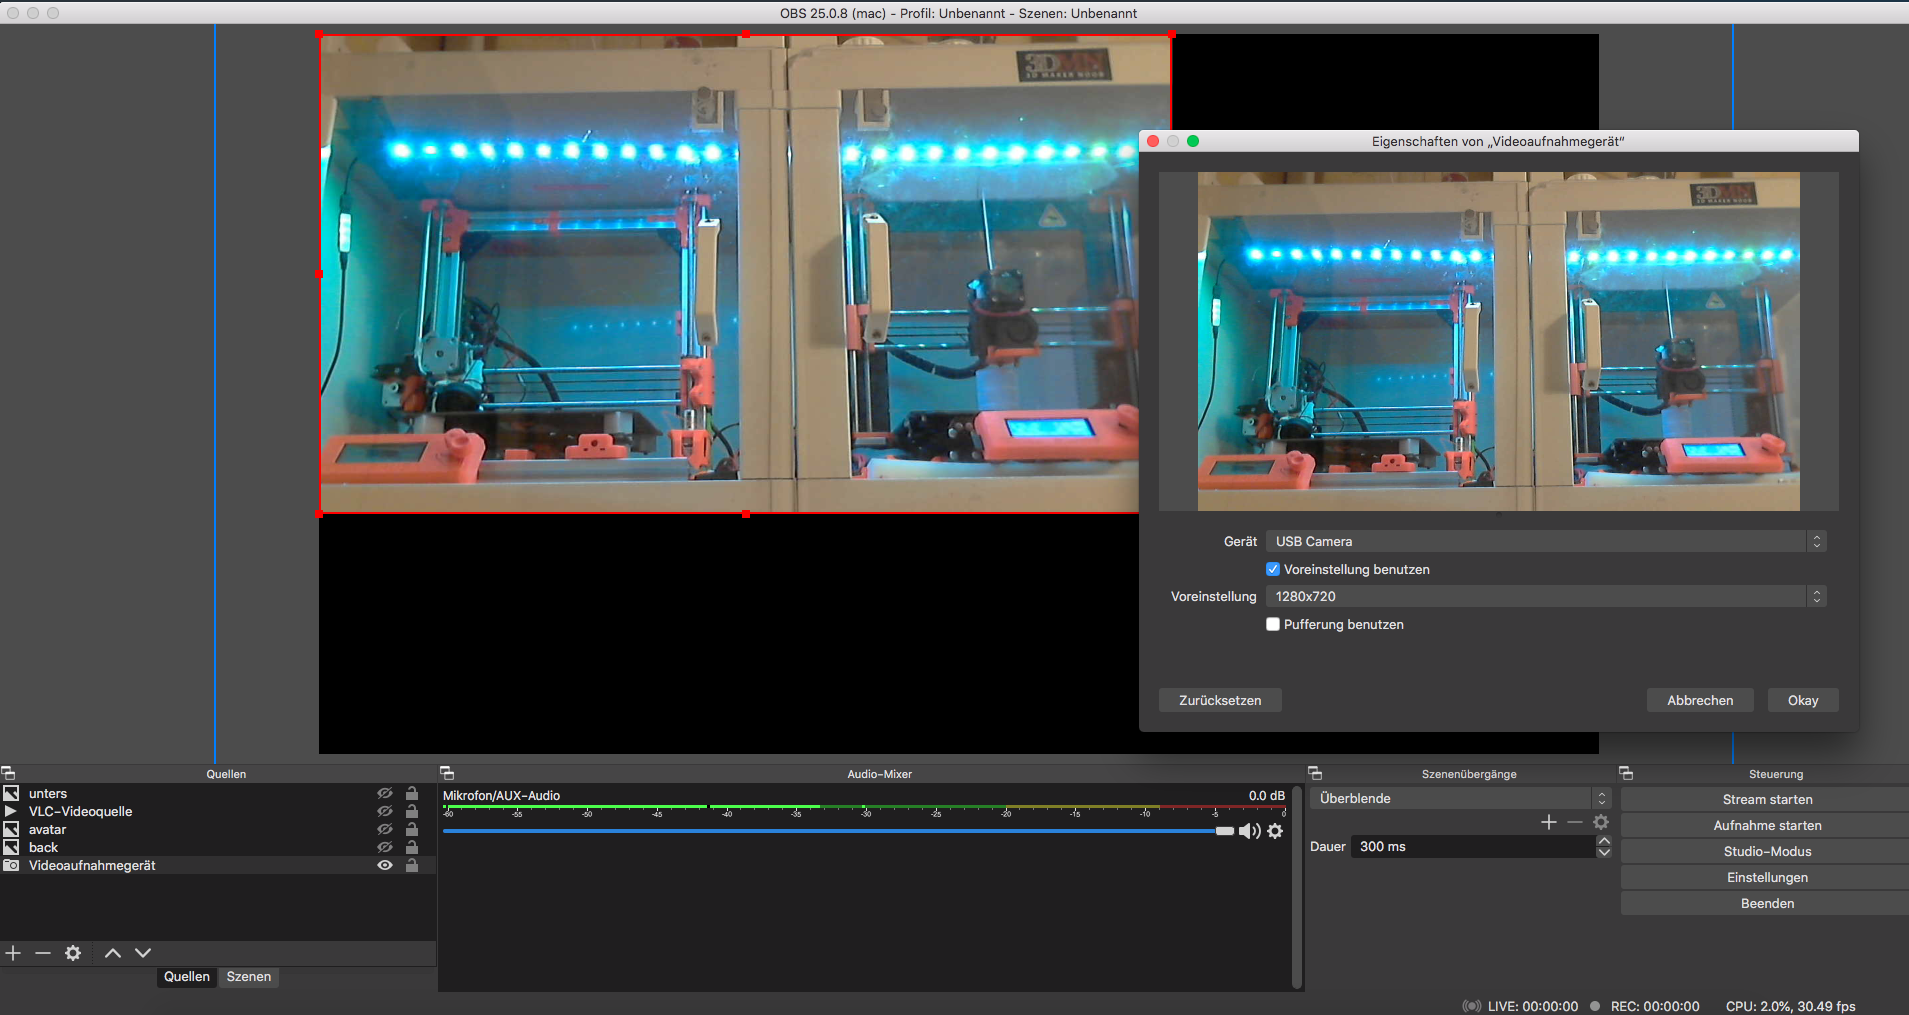
\includegraphics[width=0.9\textwidth]{./pictures/usbcamOBS.png}
\end{center}

% {\vspace{-0.6cm}}
\begin{center}
  \textbf{Hier läuft ein Film neben einem Kamera-Stream über einem Hintergrund } \\
  {\vspace{0.3cm}}
  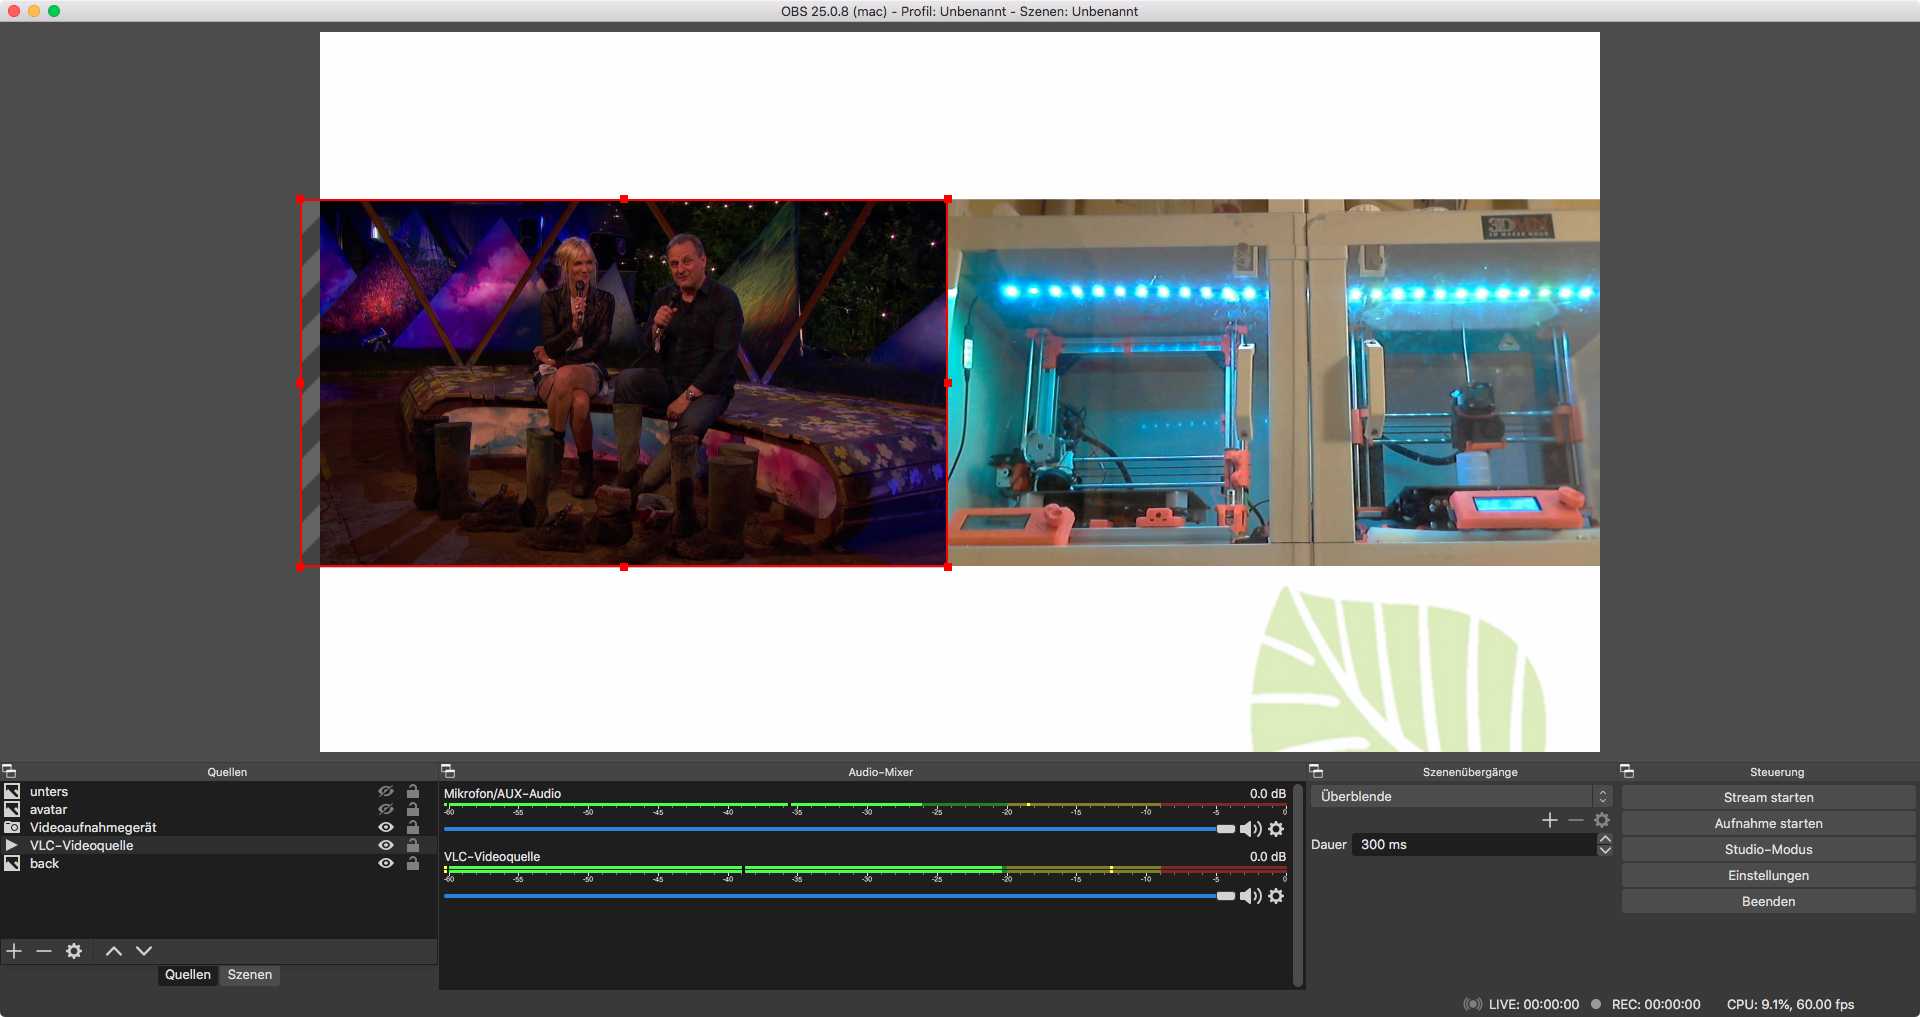
\includegraphics[width=0.7\textwidth]{./pictures/videoCAMsideBYside.png}
\end{center}
